\section{O-ISAC FOUNDATIONS AND COMPARISON FRAMEWORK}
\label{sec:foundations_comparison}
The scope defined in Section~\ref{sec:introduction} brings diverse optical
systems into one survey. This section turns that scope into a comparison
profile by following the physical context, coupling location, measurement
contract, and evidence trace of each result. Together, these elements preserve
the meaning of an observation and show how it can inform the synthesis.
Table~\ref{tab:comparison_record} condenses them into a map for the reader.
Figure~\ref{fig:native_evidence_objects} first distinguishes three evidence
objects that retain meaning through their native frames.

\begin{figure*}[!t]
\centering
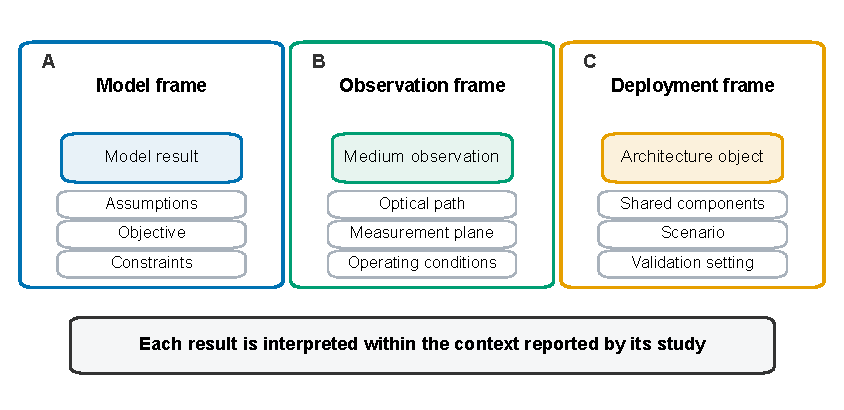
\includegraphics[width=\textwidth]{figures/final_submission_2026-08-25/fig01_native_evidence_objects.pdf}
\caption{Native evidence objects represented in O-ISAC syntheses. A model
result retains its assumptions, objective, and constraints. A medium
observation retains its optical path, measurement plane, and operating
conditions. An architecture or deployment object retains its shared
components, scenario, and validation setting. The equal panels present
parallel evidence forms whose interpretation remains tied to their native
frames.}
\label{fig:native_evidence_objects}
\end{figure*}

Each evidence form supports a distinct kind of reasoning. Reconciliation at
the study level connects them across sources by preserving the context carried
with every result.

\subsection{System Boundary, Modality, and Signal Path}

Technical comparison begins by locating communication and sensing within their
physical signal paths. The modality of the observable is recorded separately
from the hardware used to generate, distribute, or process the signal. This
distinction provides the physical reference for the six analytical families
used in the survey.

The evidence is organized into fiber, free space optical, visible light
communication and LiFi, photonic terahertz, hybrid optical, and other optical
systems. These analytical categories place each result in its relevant
physical regime before performance comparison.

Fiber systems either sense the guided path directly or use it to transport
signals to a downstream segment that reaches the target. Free space optical
systems place target geometry and beam control in a directional optical path,
while visible light communication and LiFi add illumination and access
constraints. In photonic terahertz systems, optical hardware
may generate, distribute, or process the carrier, while a radio frequency path
reaches the target. Hybrid systems combine both physical domains through their
interface. These platform boundaries guide the synthesis of study counts,
implementations, and constraints in
Section~\ref{sec:optical_modality_families}
\cite{OISAC_SCR00220,OISAC_SCR00940,OISAC_SCR00196,OISAC_SCR00083,
OISAC_SCR00366}.

\subsection{Integration Mechanisms and Measurement Planes}

Integration is located where the two functions share a component, signal,
resource, path, or decision. Application coupling can coordinate a service even
when the signal paths remain separate. At the physical and signal levels,
systems may share a link, hardware element, optical carrier, waveform, or
allocation rule. Joint design connects these choices by selecting at least one
variable using outcomes from both functions.

These locations overlap within a system. Shared hardware can support separate
waveforms, while a joint optimization model can coordinate both functions
before hardware validation. A shared hardware application
\cite{OISAC_SCR00001}, a fiber system with a shared link
\cite{OISAC_SCR00957}, and a design that combines multiple mechanisms
\cite{OISAC_SCR00220} therefore represent distinct engineering relations. We
keep these attributes separate to reveal how concurrency, resource use, and
validation differ across architectures.

The measurement plane identifies where the reported quantity is observed. Design
variables describe carrier and waveform settings, launch power, and geometry.
Optical power, loss, and optical signal to noise ratio (OSNR) belong to the
optical link. After conversion, electrical signal to noise ratio (SNR), error
rate, and throughput describe the electrical and digital stages. Sensing
measurements add observations specific to the task, including geometry, motion, environment,
classification, or detection.

Familiar labels become comparable through matched references. OSNR and
electrical SNR belong to different planes, just as launch and received power
describe different locations in the chain. Rate accounting distinguishes gross
from net data, and error accounting distinguishes the event measured before
forward error correction from the event measured after forward error correction.
Sensing likewise separates range resolution,
estimation error, precision, and analytical bounds. Comparison therefore
follows the task, target, operating point, channel, and processing chain
together with the metric name.

Provenance adds the form of evidence. Analytical bounds, simulations,
laboratory measurements, offline dataset results, and field observations
support different kinds of inference. When decisive conditions align, their
results can reveal a bounded relation across studies. Within a study, a sweep
can show how a design choice changes outcomes across its reported operating
region.

Figure~\ref{fig:comparison_framework} brings the physical context, coupling
location, measurement contract, and provenance into one comparison record. The
record then identifies the analytical use supported by the available context.

\begin{figure*}[!t]
\centering
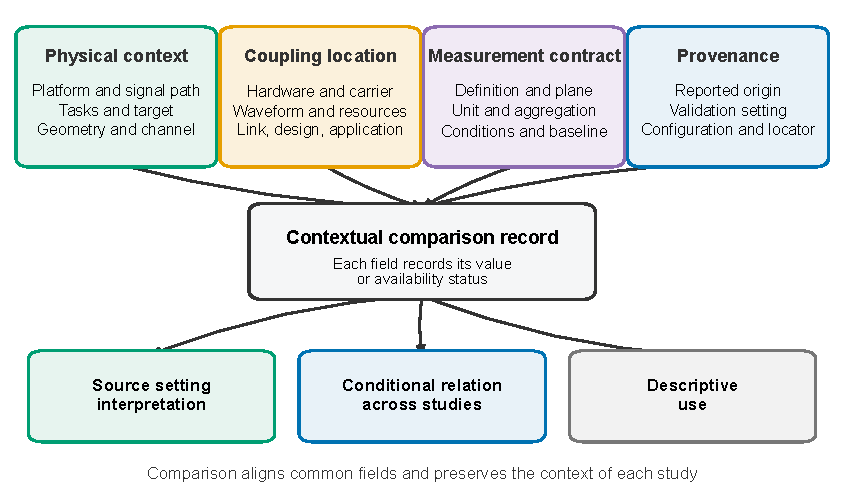
\includegraphics[width=\textwidth]{figures/final_submission_2026-08-25/fig02_comparison_framework.pdf}
\caption{Framework based on four comparison axes for interpreting O-ISAC
evidence across platforms. Physical context locates the tasks and signal path. Coupling location
records where the functions meet. The measurement contract retains the
definition, plane, unit, conditions, and baseline. Provenance retains the value
origin, validation setting, configuration, and source locator. Together, these
fields support interpretation in the source setting, a conditional relation
across studies, or descriptive placement.}
\label{fig:comparison_framework}
\end{figure*}

The four axes have equal roles in the comparison record, and the outcome states
the supported analytical use. Table~\ref{tab:comparison_record} provides the
compact field map used throughout the survey.

\begin{table}[!htbp]
\caption{Comparison profile carried with each reported O-ISAC result}
\label{tab:comparison_record}
\centering
\footnotesize
\setlength{\tabcolsep}{3.2pt}
\renewcommand{\arraystretch}{1.04}
\begin{tabularx}{\columnwidth}{@{}>{\raggedright\arraybackslash}p{0.29\columnwidth}
>{\raggedright\arraybackslash}X@{}}
\toprule
\multicolumn{2}{@{}l}{\emph{Comparison profile}} \\
\addlinespace[1pt]
Component & Context carried with the result \\
\midrule
Physical context & Modality, the signal path that reaches the target and its conversion boundary,
communication task or role, sensing task, and target locate the physical regime. \\
Coupling location & A shared component, carrier, waveform, resource, path,
application, or design rule shows where the functions meet. \\
Measurement contract & Metric name and source definition, statistic,
measurement plane, unit and accounting state, operating point, channel,
geometry, environment, reference or ground truth, constraints, and baseline
define the quantity and operating region. \\
Evidence trace & Validation setting, value origin, and exact source locator
connect the result to its evidence. \\
\bottomrule
\end{tabularx}

\vspace{3pt}
\begin{tabularx}{\columnwidth}{@{}>{\raggedright\arraybackslash}p{0.34\columnwidth}
>{\raggedright\arraybackslash}X@{}}
\toprule
\multicolumn{2}{@{}l}{\emph{Analytical use}} \\
\addlinespace[1pt]
Use & Evidence condition \\
\midrule
Interpretation within a study & The result supports a technical interpretation
under the conditions reported by its source. \\
Bounded relation across studies & Decisive fields align and the remaining
differences are stated. \\
Descriptive retention & The record informs mechanism, scope, or feasibility in
its reported context. \\
\bottomrule
\end{tabularx}
\vspace{1pt}
\parbox{\columnwidth}{\footnotesize\emph{Note.} Electronic Supplements
S-Data Dictionary and S-Evidence provide the exact field definitions,
controlled states, coding rules, and provenance for each record. The comparison
decision follows the source fields available for each result.}
\end{table}

\subsection{Comparison Profile Across Platforms}

The profile becomes comparative when its decisive fields align. A matched
definition and measurement plane establish what is being compared, while the
operating region and evidence trace state where the relation holds. This keeps
each quantitative relation tied to the physical system and the metric's
reported meaning.

One fiber study illustrates this logic. Its communication and localization
outcomes form a bounded relation under shared conditions, while its other
results retain narrower roles within their recorded settings
\cite{OISAC_SCR00056}. The profile makes each role visible and preserves the
platform context for later synthesis.

Throughout the survey, selected studies anchor recurring patterns, while tables
provide compact corpus maps.
Modality and signal path establish physical context, integration locates the
coupling, and the measurement plane identifies the observation. Together with
the evidence trace, these elements determine how evidence can be related
across studies.
